\documentclass[24pt]{beamer}

\usetheme{Jacquenetta}

% Required packages
\usepackage[utf8]{inputenc} 
\usepackage{amsmath} 
\usepackage{amsfonts}
\usepackage{amssymb} 
\usepackage{booktabs}
\usepackage{algpseudocodex}
\usepackage{xurl}
\usepackage{multicol}

\setbeamerfont{caption}{size=\tiny}

\title[LLM Optimization]{Fine-tuning, Reinforcement Learning and Parameter-Efficient Adaptation}
\author{Dimitris Tsirmpas}
\date{\today}
\institute{Athens University of Economics and Business \and Archimedes, Athena Research Center}


\begin{document}
    % =========================================================
    % SLIDE 1: Transition and Defining Fine-Tuning (0:30)
    % =========================================================
    \begin{frame}
        \titlepage
    \end{frame}
    
    
    \section{Practically Finetuning LLMs}

    \begin{frame}
        \frametitle{Why finetune LLMs?}
        \begin{itemize}
            \item \textbf{Prompting:} Changes \alert{input behavior}. We
            guide the model with instructions and examples.
            \item \textbf{Fine-Tuning:} Changes \alert{model parameters}. We
            switch the \alert{knowledge} of the model.
        \end{itemize}

       \begin{block}{Reminder}
       	\textbf{Fine-Tuning (FT):} The process of further training a pre-trained model on a smaller, domain-specific dataset to adapt its general knowledge to a specialized task.
       \end{block}
    \end{frame}

    % =========================================================
    % SLIDE 2: The Pitfall of Full Fine-Tuning (0:30 - 0:50)
    % =========================================================
    
    \begin{frame}
    	\frametitle{Why not finetune LLMs?}
    	\begin{itemize}
    		\item \textbf{High Resource Cost:}
    		\begin{itemize}
    			\item \textbf{Computational Power:} Full FT requires massive and thousands of compute hours for large models (e.g.,
    			Llama-70B). 
    			
    			\item \textbf{Storage:} Each specialized task
    			requires a separate, full copy of the massive foundational
    			model.
    		\end{itemize}
    	\end{itemize}
    \end{frame}
    
    \begin{frame}
    	\frametitle{Why not finetune LLMs?}
    	\begin{itemize}
    		\item \textbf{Operational Overhead:}
    		\begin{itemize}
    			\item Training is \alert{slow}. 
    			\item Deployment becomes complex,
    			managing \alert{multiple large models} for different applications.
    			\begin{itemize}
    				\item A single 13B model may require 26GB of storage.
    				\item 10 finetuned models may thus require 260GB.
    			\end{itemize}
    			\item High risk of \alert{Catastrophic Forgetting}---the model forgets
    			its general knowledge while learning the specific task.
    		\end{itemize}
    	\end{itemize}
    	
    \end{frame}
    
    \begin{frame}
    	\frametitle{Why not finetune LLMs?}
    		\begin{columns}
    			
    			\begin{column}{0.45\textwidth}
    				\begin{block}{BERT}
    					\centering
    					\begin{itemize}
    						\item \textbf{Model Size:} $\sim$340M Parameters 
    						\item \textbf{VRAM Requirement:} $\approx$ 8-12GB
    						\item \textbf{Training Time:} Minutes to a few hours
    					\end{itemize}
    				\end{block}
    			\end{column}
    		
	    		\begin{column}{0.45\textwidth}
	    			\begin{block}{Llama 70B}
	    				\centering
	    				\begin{itemize}
	    					\item \textbf{Model Size:} $\sim$70 Billion Parameters
	    					\item \textbf{VRAM Requirement:} $\approx$1000GB+
	    					\item \textbf{Training Time:} Days to Weeks (even with specialized hardware)
	    				\end{itemize}
	    			\end{block}
	    		\end{column}
    	\end{columns}
    	
    	\begin{center}
    		LLMs are \alert{too large} to run full-finetuning. But do we need to?
    	\end{center} 
    \end{frame}


    \section{Parameter Efficient Fine-Tuning (PEFT)}
    
    \begin{frame}
    	\frametitle{Parameter-Efficient Fine-Tuning (PEFT)}
    	
    	\begin{itemize}
    		\item Instead of finetuning the whole model, why not finetune \alert{only a small part}?
    		 \begin{itemize}
    		 	\item Similar in concept to finetuning a classification head.
    		 	\item Introduce and train a	tiny number of new, small matrices.
    		 \end{itemize}
    		 \item \textbf{Goal:} Achieve performance benefits
    		 of Fine-Tuning while \alert{drastically reducing the computational burden}.
    	\end{itemize}
    \end{frame}
    
    \begin{frame}
    	\frametitle{PEFT: LoRA}
    	
    	\begin{itemize}
    		\item Low-Rank (LoRA) Matrix Decomposition is a specific PEFT algorithm that exploits the fact that weight updates in LLMs have a \alert{``low intrinsic rank''}.\note{Think of it this way: imagine you have a large spreadsheet with 1,000 rows and 1,000 columns (1 million cells total). If you need to update this spreadsheet, but the updates follow certain patterns, you might be able to represent all those changes using just two smaller lists: one with 1,000 numbers and another with 8 numbers. By mathematically combining these lists, you can reproduce the effect of updating the million-cell spreadsheet while only storing 1,008 numbers instead of 1,000,000.}
    		
    		\item Low rank matrices enable us to \alert{scalably} represent information.
    	\end{itemize}
    	
    	\[
    	\begin{bmatrix}
    		2 & 4 & 6 & 8 & 10\\
    		1 & 2 & 3 & 4 & 5\\
    		3 & 6 & 9 & 12 & 15\\
    		4 & 8 & 12 & 16 & 20
    	\end{bmatrix}
    	=
    	\begin{bmatrix}
    		2\\
    		1\\	
    		3\\
    		4
    	\end{bmatrix}
    	\begin{bmatrix}
    		1 & 2 & 3 & 4 & 5
    	\end{bmatrix}.
    	\]

    \end{frame}
    
    
    \begin{frame}
    	\frametitle{LoRA: Low-rank decomposition}
    	
    	\[
    	\underbrace{
    		A_{m \times n}
    	}_{\text{large matrix}}
    	\approx
    	\underbrace{
    		U_{m \times r}
    	}_{\text{left factors}}
    	\underbrace{
    		V_{r \times n}
    	}_{\text{right factors}},
    	\qquad r \ll \min(m,n).
    	\]
    	
    	 \[
    	A_{10000 \times 5000}
    	\approx
    	U_{10000 \times 50}
    	V_{50 \times 5000},
    	\]
    	
    	\[
    	\underbrace{10000 \times 5000}_{50,000,000\ \text{parameters}}
    	\;\longrightarrow\;
    	\underbrace{10000 \times 50 + 50 \times 5000}_{750,000\ \text{parameters}}.
    	\]
    \end{frame}
    
    
    \begin{frame}
    	\frametitle{LoRA: Mathematical Foundation}
    	
    	\begin{figure}
    		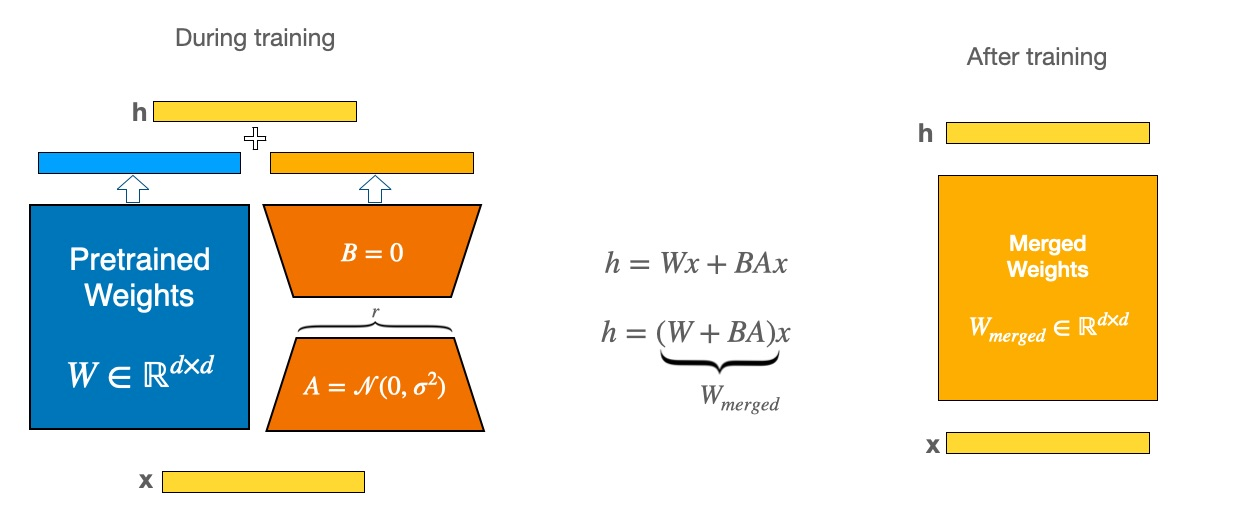
\includegraphics[width=0.8\textwidth]{LoRA.jpeg}
    		\centering
    		\caption{\url{https://huggingface.co/docs/peft/main/conceptual_guides/lora}}
    	\end{figure}
    	
    	\begin{multicols}{2}
    		\begin{itemize}
    			\item $W \in \mathbb{R}^{d \times k}$ weights.
    			\item $x$ input, $h$ output.
    			\item We add $BAx$ to the output.
    			\item $B  \in \mathbb{R}^{d \times r} \rightarrow$ zeros.
    			\item $A \in \mathbb{R}^{r \times k} \rightarrow$ Gaussian.
    			\item $r \ll \min(d, k)$, hence $A, B$ are much smaller than $W$.
    		\end{itemize}
    	\end{multicols}
    		
    \end{frame}
    
    
    \begin{frame}
    	\frametitle{LoRA: Algorithm}
    	
		\begin{algorithmic}
			\LComment{====Initialization====}
			\ForAll{$W \in all\_weights$}
				\State Set $\mathbf{W}$ to read-only \Comment{Original knowledge preserved}
			\EndFor
			
			\ForAll{$W_u \in target\_modules$}
				\State Initialize $\mathbf{A}$ randomly
				\State Initialize $\mathbf{B} = \mathbf{0}$ \Comment{Contributes zero to the output initially}
			\EndFor
			
			\LComment{====Backpropagation====}
			\ForAll{$X \in input\_embeds$}
				\State $\mathbf{\Delta W} = \frac{\alpha}{r} \mathbf{A} \mathbf{B}$
				\State $\mathbf{H} = \mathbf{W} X + \mathbf{\Delta W} X$ \Comment{Output = original + adaptation}
			\EndFor
			\LComment{====End of training====}
			\State $\mathbf{W}' = \mathbf{W} + \frac{\alpha}{r} (\mathbf{A} \mathbf{B})$ \Comment{Merge original and adaptation}
		\end{algorithmic}
	\end{frame}
	
	\begin{frame}
		\frametitle{LoRA: Practical Considerations}
		
		\begin{itemize}
			\item How many ranks do I use?
			\begin{itemize}
				\item $r \in [1,16]$: fast, easy, recommended for minor adjustments.
				\item $r \in [16,64]$: recommended for most domain adaptation scenarios.
				\item $r \in [64, 256]$: may hit computational bottlenecks, only use for  dramatic shifts in domain and knowledge.
			\end{itemize}
			
			\item How do I set $\alpha$?
			\begin{itemize}
				\item Usually set to a multiple of $r$ .
				\item Very low $\alpha \rightarrow$ minimal contribution. Very high $\alpha \rightarrow$ destruction of model knowledge.
				\item $\alpha = 2r$ usually used as a starting point.
			\end{itemize}
		\end{itemize}
		
	\end{frame}
	
	\begin{frame}
		\frametitle{LoRA: Practical Considerations}
		
		\begin{itemize}
			\item What modules do I change?
			\item Start from the top of this list and go down as required:
			\begin{enumerate}
				\item \textbf{Query ($\text{q\_proj}$) and Value ($\text{v\_proj}$):} Most frequently adapted; control \alert{how the model attends} to input.
				\item \textbf{Key ($\text{k\_proj}$):} Increases \alert{information retrieval} capacity.
				\item \textbf{Output ($\text{o\_proj}$):} Less common, but useful for modifying \alert{integrated} attended information.
				\item \textbf{Feed-forward Networks (MLP):} Possible to adapt, but generally offer less parameter benefit compared to attention layers.
			\end{enumerate}
		\end{itemize}
		
	\end{frame}
	
	\begin{frame}
		\frametitle{LoRA: Limitations}
		
		\begin{itemize}
			\item The largest limitation to LoRA is \alert{memory} and \alert{inference} costs.
			\begin{itemize}
					\item While LoRA makes training the model easier, it does not change the fact that we still need to \alert{load a very large model}.
				\item Training small models still requires enterprise-grade GPUs.
				\item During inference, there is essentially \alert{no gain in performance}.
			\end{itemize}
			\item The solution to large models is making them smaller $\rightarrow$ \alert{quantization}.
		\end{itemize}
	\end{frame}

	
    \begin{frame}
    	\frametitle{QLoRA: Quantization}
    	
    	\begin{columns}
    		\begin{column}{0.45\textwidth}
    			\begin{itemize}
    			\item Quantization refers to dropping the size (not number) of the LLM parameters.
    			
    			\item Normally, each parameter is stored in a 16 bit floating point.
    			
    			\item Quantization can drop them to usually 4 bits, resulting in $\times 4$ less GPU memory and inference costs.
    			
    			\end{itemize}
    		\end{column}
    		
    		\begin{column}{0.45\textwidth}
    			\begin{figure}
    				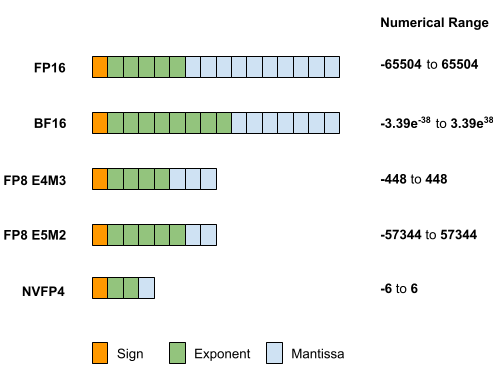
\includegraphics[width=\columnwidth]{quantization-fp.png}
    				\centering
    				\caption{\url{https://developer.nvidia.com/blog/model-quantization-concepts-methods-and-why-it-matters}}
    			\end{figure}
    		\end{column}
    	\end{columns}
    \end{frame}
    
    
    \begin{frame}
    	\frametitle{QLoRA: Quantization}
    	
    	\begin{columns}
    		\begin{column}{0.45\textwidth}
    			\begin{itemize}
    				\item Quantization is one of the \alert{most useful tools} at your disposal.
    				
    				\item Allows for training and inference in consumer-grade hardware.
    				
    				\item We will return to this in Module 5.
    				
    			\end{itemize}
    		\end{column}
    		
    		\begin{column}{0.45\textwidth}
    			\begin{figure}
    				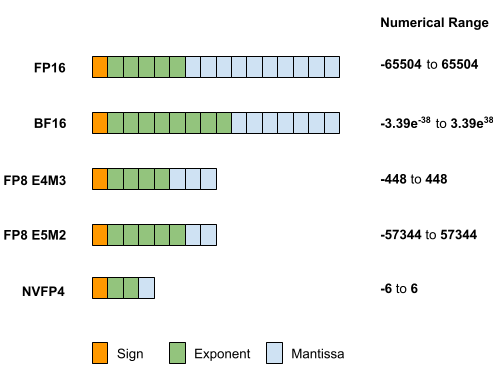
\includegraphics[width=\columnwidth]{quantization-fp.png}
    				\centering
    				\caption{\url{https://developer.nvidia.com/blog/model-quantization-concepts-methods-and-why-it-matters}}
    			\end{figure}
    		\end{column}
    	\end{columns}
    \end{frame}
    
    \begin{frame}
    	\frametitle{QLoRA: Concept}
    	
    	\begin{columns}
    		\begin{column}{0.45\textwidth}
    			\begin{itemize}
    				\item Load a 4-bit quantized model using a normal approximation of weights.
    				
    				\item Run LoRA in full precision, \alert{dequantizing} the model weights \alert{one at a time}.
    				
    				\item Continue as normal.
    				
    			\end{itemize}
    		\end{column}
    		
    		\begin{column}{0.45\textwidth}
    			\begin{figure}
    				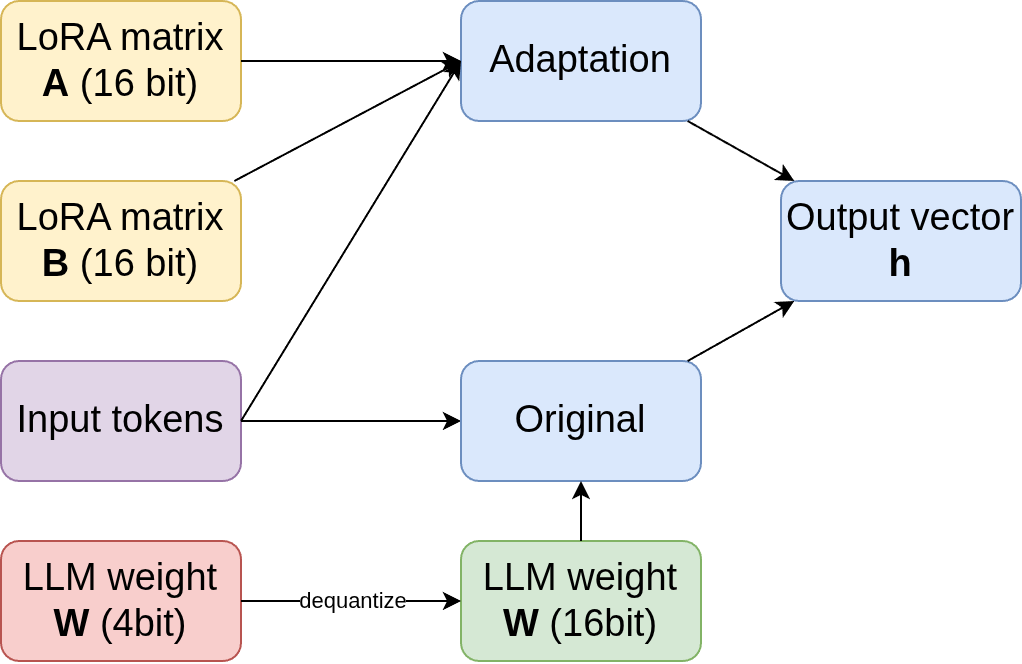
\includegraphics[width=\columnwidth]{qlora.drawio.png}
    				\centering
    			\end{figure}
    		\end{column}
    	\end{columns}
    \end{frame}
    
    \begin{frame}
    	\frametitle{QLoRA: Algorithm}
    	
    	\begin{algorithmic}
    		\LComment{====Initialization====}
    		\LComment{Same as before}
    		
    		\LComment{====Backpropagation====}
    		\ForAll{$X \in input\_embeds$}
    		\State $\mathbf{\Delta W} = \frac{\alpha}{r} \mathbf{A} \mathbf{B}$
    		\State $\mathbf{H} =$ \Call{dequant}{$\mathbf{W}$} $X + \mathbf{\Delta W} X$ \Comment{Output = original + adaptation}
    		\EndFor
    		\LComment{====End of training====}
    		\LComment {Only attempt dynamic merge. Ignore this advice at your own peril, or if you really know what you are doing.}
    	\end{algorithmic}
    \end{frame}
    
\end{document}
